%!TEX root = paper.tex

\section{Example}

We have implemented an experimental research testbed for training agents using this approach (Figure \ref{horde}), written with the MASON multiagent simulation toolkit \cite{luke:simulation:2005}.
%%% Commented out for anonymity
%(see  {\sf http:/\!/cs.gmu.edu/\(\sim\)eclab/projects/mason/}).   
In the environment, our agent can sense a variety of things: the relative locations of obstacles, other agents of different classes, certain predefined waypoints, food locations, etc.  In this testbed, the experimenter trains an HFA by first selecting features relevant to the behaviors (see Figure \ref{features}), then grounding targets for behaviors and features, then directing the agent to perform behaviors by pressing various buttons or keystrokes, and then finally adding the trained HFA to the system library.



\begin{figure}[t]
\begin{center}
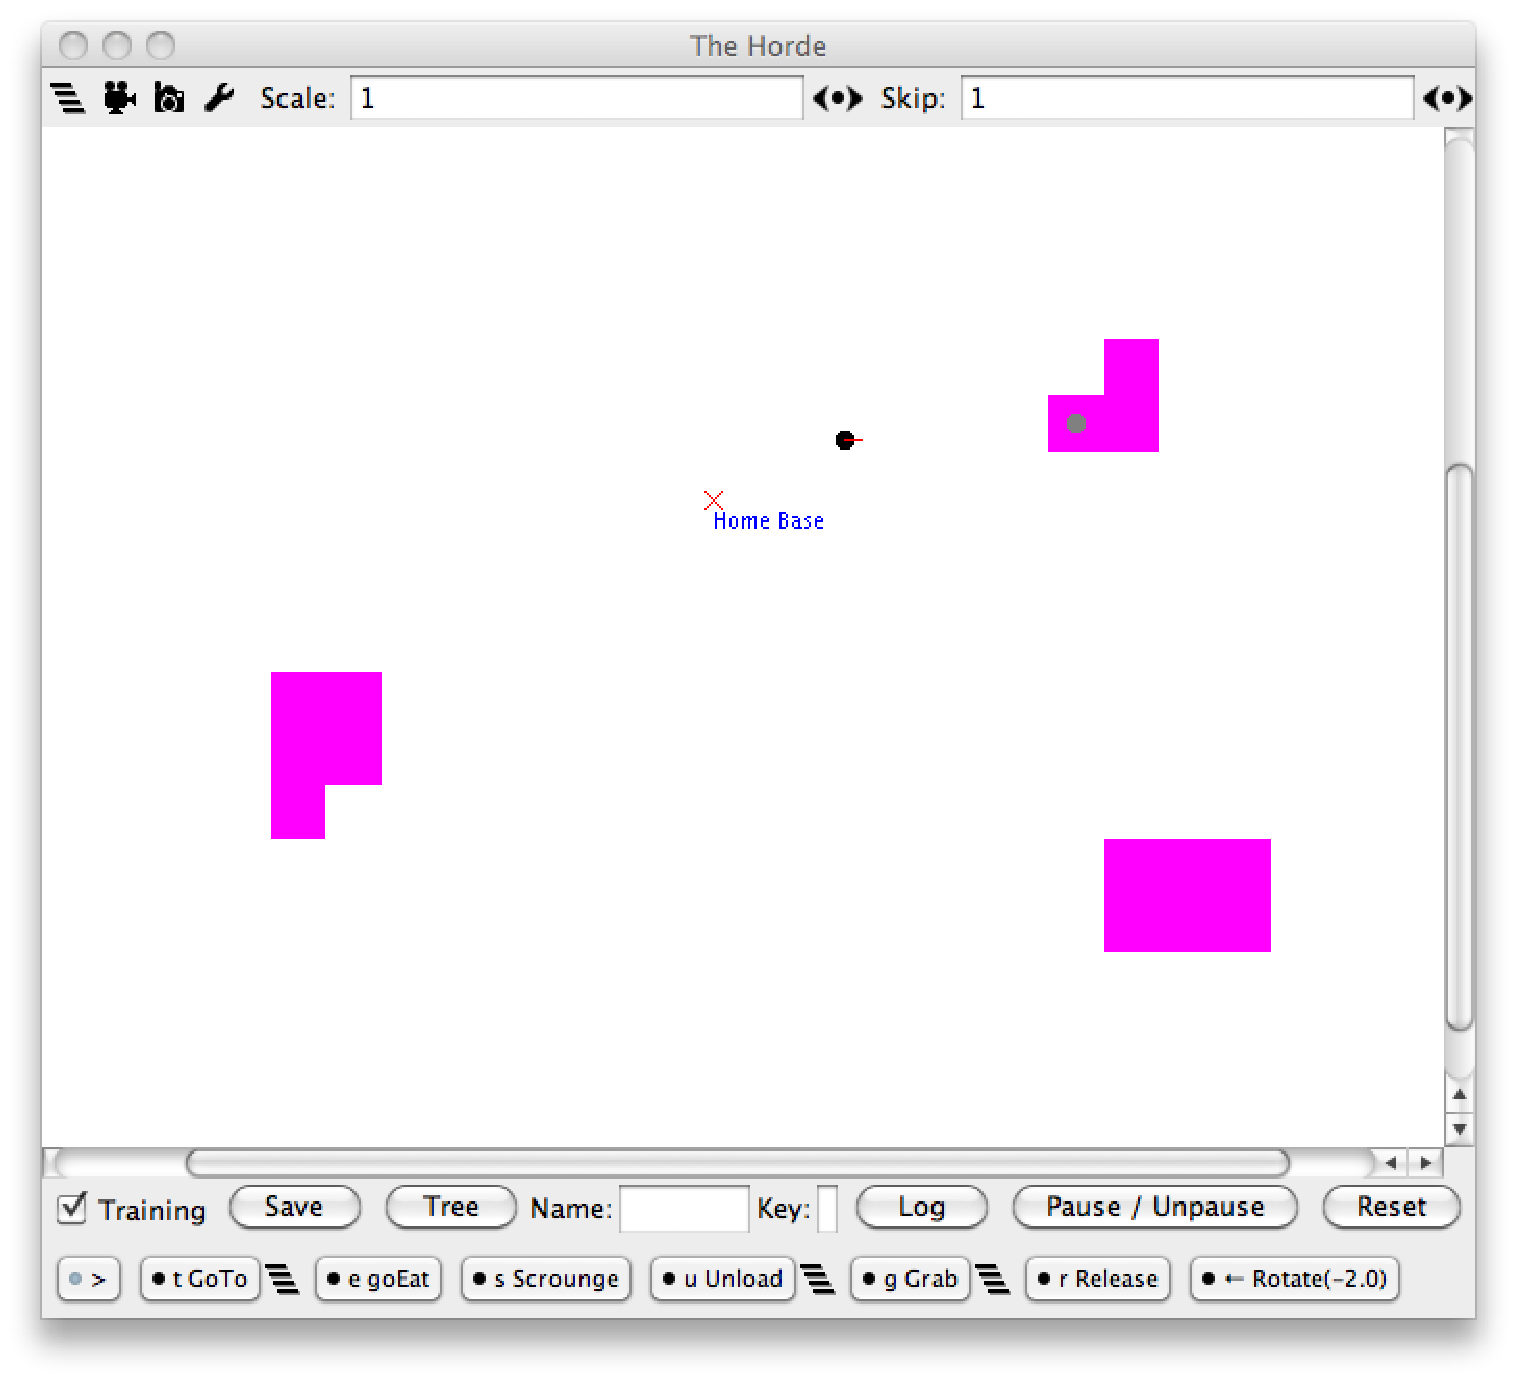
\includegraphics[width=3.3in]{ForagingHorde.pdf}
\end{center}
\caption{The foraging scenario in our testbed.}
\label{horde}
\end{figure}



We have successfully trained several simple behaviors, tracking and acquiring a target, wall-following, generic obstacle circumnavigation, and tracing paths (such as a figure eight path between two targets).  In this section,  we give an example where we have trained the agent to perform a moderately complex foraging task: to harvest food from food sources and bring it back to deposit at the agent's central station.  Food can be located anywhere, as can the station. Food at a given location can be in any concentration, and depletes, eventually to zero, as it is harvested by the agent.  The agent can only store so much food before it must return to the station to unload.  There are various corner cases: for example, if the agent depletes food at a harvest location before it is full, it must continue harvesting at another location rather than return to the station. The scenario is shown in Figure \ref{horde}: the black circle is the agent, pink areas are food sources, and the red ``\(\times\)'' (labelled ``Home Base'') is the station.

\begin{figure}[t]
\begin{center}
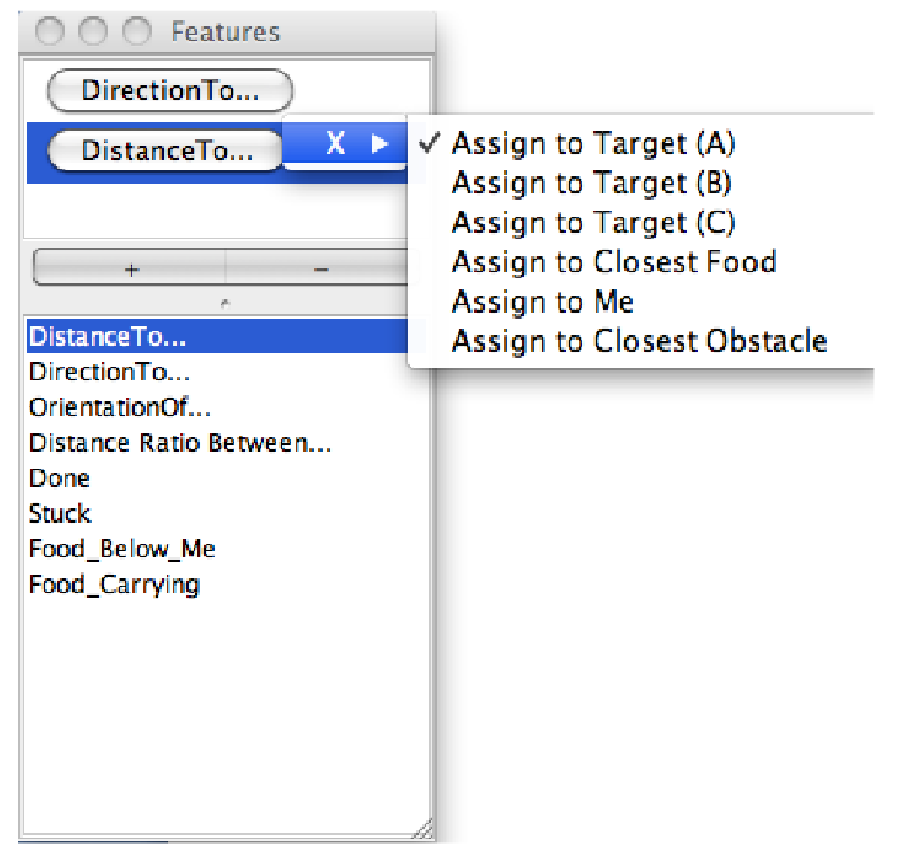
\includegraphics[width=2.5in]{Features.pdf}
\end{center}
\caption{Feature selection and target assignment.}
\label{features}
\end{figure}

\begin{figure*}[t]
\begin{center}
\noindent\begin{tabular}{cc}
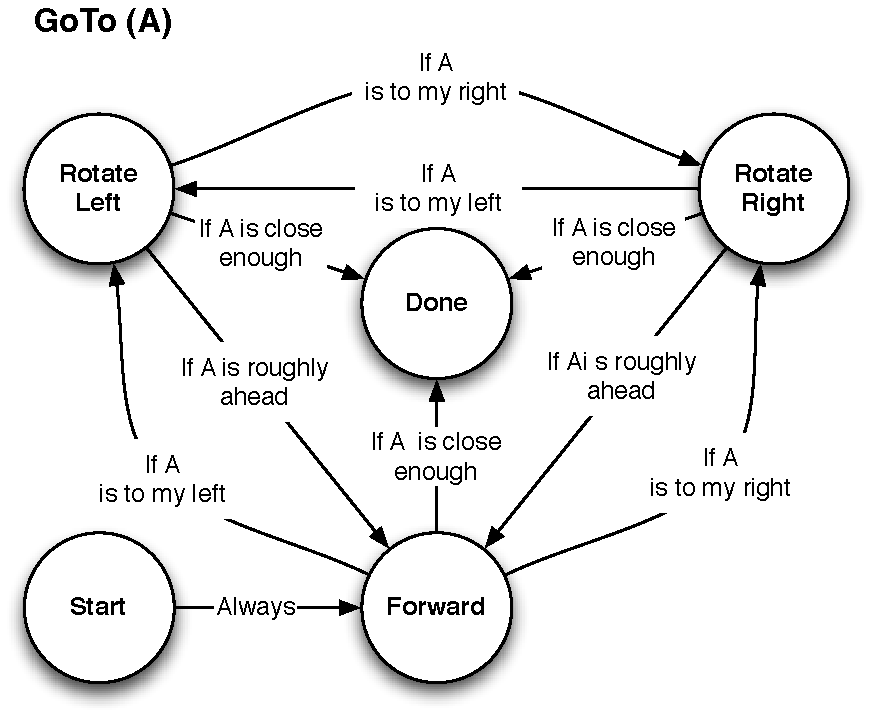
\includegraphics[width=3.5in]{GoTo.pdf}&
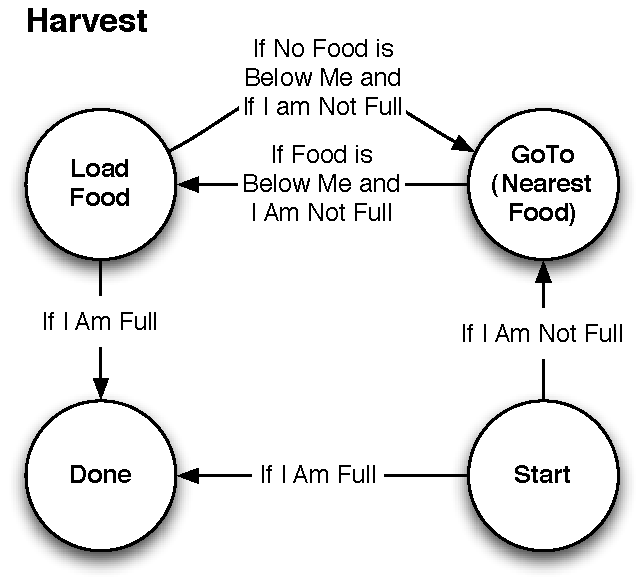
\includegraphics[width=2.6in]{Harvest.pdf}\\
\\
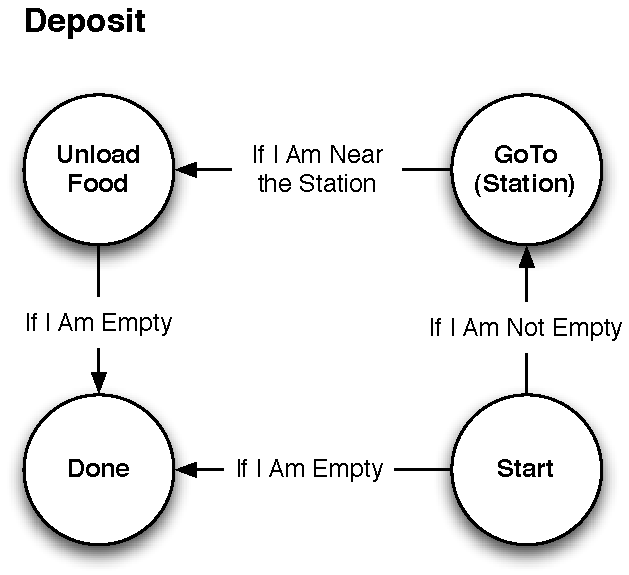
\includegraphics[width=2.6in]{Deposit.pdf}&
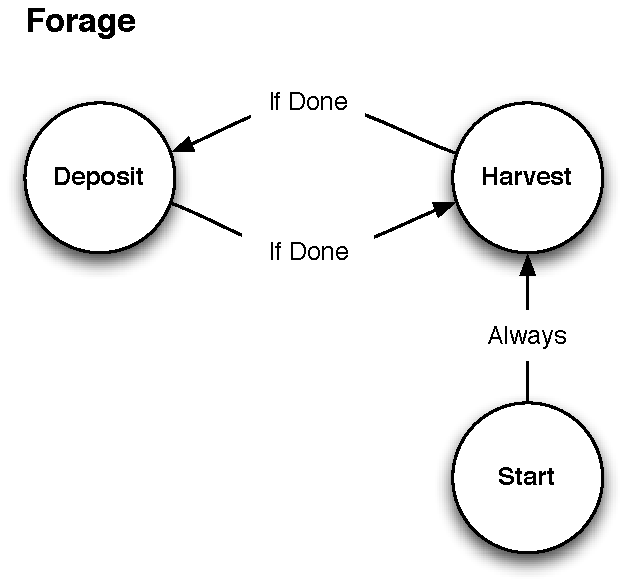
\includegraphics[width=2.6in]{Forage.pdf}\\
\end{tabular}
\end{center}
\caption{The Forage behavior and its sub-behaviors: Deposit, Harvest, and GoTo(\textit{Parameter} A).  All conditions not shown are assumed to indicate that the agent remain in its current state.}
\label{foraging}
\end{figure*}




Foraging tasks are of course old hat in robotics, and are not particularly difficult to code by hand.  But {\it training} such a behavior is less trivial.  We selected this task as an example because it illustrates a number of features special to our approach: our foraging behavior is in fact a three-layer HFA hierarchy; employs ``done'' states; involves real-valued, toroidal, and categorical (boolean) inputs; and requires one behavior with an unbound parameter used in two different ways.

The behavior is shown in Figure \ref{foraging}.  It requires seven basic behaviors: \textsf{start} and \textsf{done},  \textsf{forward}, \textsf{rotate-left}, \textsf{rotate-right}, \textsf{load-food} (deplete the current location's food by 1, and add 1 to the agent's stored food), and \textsf{unload-food} (remove all the agent's stored food).  It also requires several features: \textsf{distance-to(A)}, \textsf{angle-to(A)}, \textsf{food-below-me} (that is, how much food is located here), \textsf{food-stored-in-me}, and \textsf{done}.  Finally, it requires two targets to bind to A: the \textsf{station} and \textsf{nearest-food}.  

From this we decomposed the foraging task into a hierarchy of four HFA behaviors, and trained each one in turn as described next.  All told, we were able to train all four behaviors, and demonstrate the agent properly foraging, in a manner of minutes.

\paragraph*{The GoTo(A) Behavior} This behavior caused the agent to go to the object marked A.  The behavior was a straightforward bang-bang servoing controller: rotate left if A is to the left, else rotate right if A is to the right; else go forward; and when close enough to the target, enter the ``done'' state.
 
We trained the GoTo(A) behavior by temporarily declaring a marker in the environment to be Parameter A, and reducing the features to just \textsf{distance-to(A)} and \textsf{angle-to(A)}.  We then placed the agent in various situations with respect to Parameter A and ``drove'' it over to A by pressing keys corresponding to the \textsf{rotate-left}, \textsf{rotate-right}, \textsf{forward}, and \textsf{done} behaviors.  After a short training session, the system quickly learned the necessary behaviors to accurately go to the target and signal completion.  Once completed, it was made available in the library as \textsf{go-to(A)}.

\paragraph*{The Harvest Behavior} This behavior caused the agent to go to the nearest food, then load it into the agent.  When the agent had filled up, it would signal that it was done.  If the agent had not filled up yet but the food has been depleted, the agent would search for a new food location and continue harvesting.  This behavior employed the previously-learned \textsf{go-to(A)} behavior as a subsidiary behavior, binding its Parameter A to the \textsf{nearest-food} target.  This behavior also employed the features \textsf{food-below-me}, \textsf{food-stored-in-me}.

We trained the Harvest Behavior by directing the agent to go to the nearest food, then load it, then (if appropriate) signal ``done'', else go get more food.  We also placed the agent in various corner-case situations (such as if the agent started out already filled up with food).  Again, we were able to rapidly train the agent to perform harvesting.  Once completed, it was made available in the library as \textsf{harvest}.

\paragraph*{The Deposit Behavior} This behavior caused the agent to go to the station, unload its food, and signal that it is done.  If the agent was already empty when starting, it would immediately signal done.   This behavior also used the previously-learned \textsf{go-to(A)} behavior as a subsidiary state behavior, but instead bound its Parameter A to the \textsf{station} target.  It used the features \textsf{food-stored-in-me} and \textsf{distance-to(station)}.  We trained the Deposit Behavior in a similar manner as the Harvest Behavior, including various corner cases.  Once completed, it was made available in the library as \textsf{deposit}.

\paragraph*{The Forage Behavior} This simple top-level behavior just cycled between depositing and harvesting. Accordingly, this behavior employed the previously-learned \textsf{deposit} and \textsf{harvest} behaviors.  The behavior used only the \textsf{done} feature.
